\documentclass{ecuthesis}

% For graphics
\usepackage{graphicx}

% Bibliography
\bibliography{fullrefs,websites,patents}

% Setup the variables for the title page
\title{Using traffic analysis to identify The Second Generation Onion Router}
\author{John Barker}
\department{School of Computer and Security Science}
\school{Edith Cowan University}
\degree{Computer Science (Honours)}
\email{jebarker@our.ecu.edu.au}
\studentid{0991300}
\supervisor{Dr Andrew Woodward}
\supervisor{Mr Peter Hannay}
\supervisor{Mr Patryk Szewczyk}

% Begin document
\begin{document}
\maketitle

\tableofcontents
\listoftables
\listoffigures

\begin{abstract}
\thispagestyle{empty}

Anonymous networks provide security for users by obfuscating messages with
encryption and hiding communications amongst cover traffic provided by other
network participants. The traditional goal of academic research into these
networks has been attacks that aim to uncover the identity of network users.
But the success of an anonymous network relies not only on it's technical
capabilities, but on adoption by a large enough user base to provide adequate
cover traffic. If anonymous network nodes can be identified, the users
can be harassed, discouraging participation. Tor is an example of widely used
anonymous network which uses a form of Onion Routing to provide low latency
anonymous communications. This thesis demonstrates that traffic from a simulated
Tor network can be distinguished from regular encrypted traffic, suggesting that
real world Tor users may be vulnerable to the same analysis.

\end{abstract}

\chapter{Introduction}

\section{Background}

The first anonymous digital network, commonly known as MixNet was proposed by
\citeauthor{Chaum:1981p296} in \citetitle{Chaum:1981p296}
\parencite{Chaum:1981p296}. This paper introduced a concept integral to many
future anonymity providing designs, an intermediate system responsible for
delivering messages without the identifying details of correspondents. The
intermediate system, referred to as a 'mix' also employed public key
cryptography to ensure that eavesdroppers could not obtain delivery information.

This seminal paper spurred research into new techniques for providing anonymity
and privacy for digital networks. Remailers such as Babel
\parencite{Gulcu:1996p1662} and Mixminion \parencite{Danezis:2003ys} employed a
mix to deliver anonymous email. Research produced designs that yielded
mathematically provable anonymity
\parencite{Chaum:1988p5869,Waidner:1989p5870,Berman:2004p303} and networks that
degrade gracefully when subject to attack, so called robust anonymity
\parencite{Waidner:1989p5870,Jakobsson:1998p5137}. Designs such as MorphMix
\parencite{Rennhard:2002p4559}, Tarzan \parencite{Freedman:2002kx} and P5
\parencite{P5Sherwood:2005p5872} aimed to provide anonymity features to
peer-to-peer (P2P) networks.

Providing resistance to blocking or censorship comes in many forms. The People's
Republic of China operates a sophisticated Internet firewall capable of blocking
requests to forbidden information \parencite{The-OpenNet-Initiative:2009uq}.
This system is often referred to as the Great Firewall of China. Resisting this
system can involve ignoring spurious reset packets injected into the stream of
forbidden communications \parencite{springerlink:10.1007/11957454_2}, or be as
simple as accessing data through an encrypted proxy as is done in FreeGate
\parencite{Smart:2008kx}.

More sophisticated circumvention tend to be based on anonymity providing
designs, \textcite{Kopsell:2004:ABR:1029179.1029197} describes a censorship
resistant system built on top of AN.ON
\parencite{springerlink:10.1007/3-540-44702-4_7}. Publishing systems such as
Freedom \parencite{Goldberg:1999p2231} and Freenet \parencite{Clarke:2001p2435}
aim to provide censorship resistance as well as anonymity. Infranet uses
steganography to hide sensitive messages in innocuous content Infranet
\parencite{Feamster:2002p307}.

The Second Generation Onion Router (Tor), is an anonymous network which uses a
variant of Onion Routing, to provide low latency anonymous communications to a
wide variety of Internet communications protocols
\parencite{Dingledine:2004p314}. It also aims to provide resistance against
censorship based blocking attempts \parencite{Dingledine:2008p1542}.

\section{The Second Generation Onion Router}

Onion routing was originally developed by the U.S. Naval Research Lab in 1996
\parencite{Goldschlag:1996wy} for application by the U.S. Navy. Like a mix,
messages sent over an onion routing network were encrypted with their routing
information and delivered to an intermediate server for forward delivery.
Unlike the mix however, messages delivered using the onion routing network were
encrypted multiple times, each 'layer' using a different key and routing
instructions. The first node in a chain would only be able to encrypt the
routing instructions to deliver the message to the next node. Each node in the
sequence decrypting a layer until the complete message is decrypted and
transmitted to the destination. This invention was granted a patent by the U.S.
Patent Office in 2001 \parencite{Michael:2001}.

This proposal was expanded on in \citetitle{Dingledine:2004p314} and addressed a
number of weaknesses in the original onion router proposal
\parencite{Dingledine:2004p314}. It also added some usability and anonymity
features and deviates sufficiently from the original onion routing design in
order to avoid patent claims. The technique employed by Tor is known as
telescopic onion routing.

Tor is developed and maintained  by The Tor Project, Inc. and is made publicly
available, finding usage in journalism, law enforcement, activism and military
applications \parencite{The-Tor-Project-Inc.:2011uq}. Tor is one of the most
successful and widely deployed anonymous networks, with an average of two
hundred thousand active users as of March 2011
\parencite{The-Tor-Project-Inc.:2011fk}.

Traffic enters the Tor network through an onion proxy which accepts TCP streams.
Some identifying features are scrubbed from the data using application filters
before the data is relayed over the network through TLS \parencite{website:TLS}
encrypted connections. The intermediate nodes responsible for routing messages
are known as relays and are typically chained together to construct a circuit.
When traffic leaves the Tor network it is delivered by a special kind of relay
known as an exit node. At an exit node the data is transmitted in the original
format it was supplied to at the onion proxy.

Figure \ref{tor-network} shows the typical path a message takes through the Tor
network.

\begin{figure}[H]
  \centering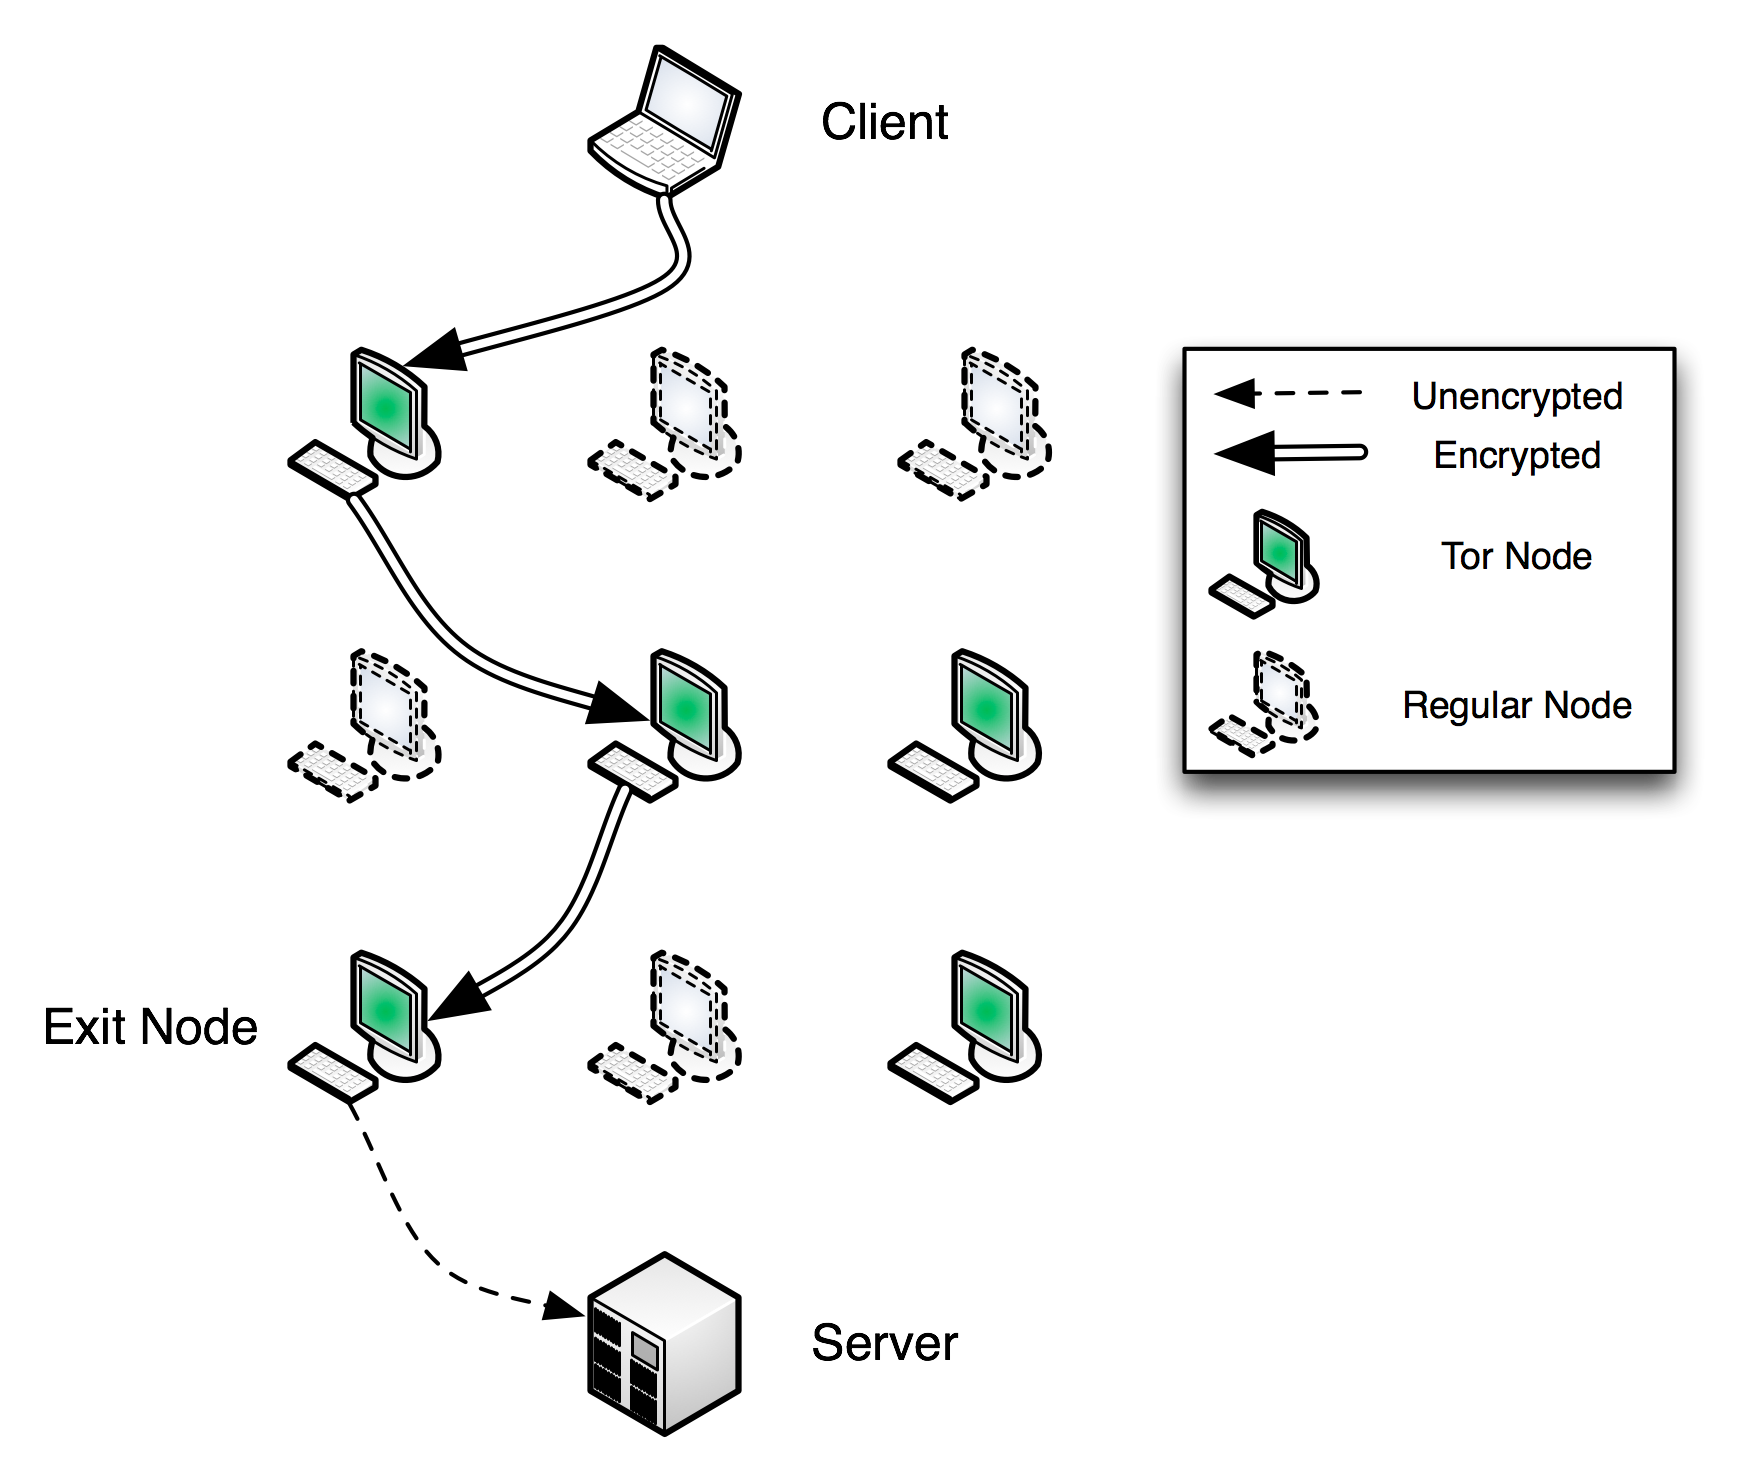
\includegraphics[width=\linewidth]{tor-network-diagram}
  \caption{The Tor Network}
  \label{tor-network}
\end{figure}

The onion proxy builds circuits incrementally, first obtaining a session key
from each successive relay in a circuit. Once all session keys for a circuit
have been obtained, the message is broken into fixed sized cells of 512 bytes
and iteratively encrypted using the session key of each node in the circuit in
the reverse order that the data traverses the network. Cells come in two forms:
control cells and relay cells. Control cells are used to create and maintain
circuits, while relay cells contain commands for circuit maintenance and
additional data for verifying message integrity and identifying streams.

When the first node in the circuit receives a cell, it removes a layer by
decrypting the message using it's session key. The cell is delivered along the
circuit and at each node a layer is removed until the cell is completely
decrypted and can be delivered successfully. Since circuits can take some time
to build, they are pre-emptively created at regular intervals
\parencite[5]{Dingledine:2004p314}.

\section{Vulnerabilities and Weaknesses}

When designing a system such as Tor, a number of trade-offs have to be made
between the strength of the security provided and the convenience and
performance of the system. The Tor designers consciously prioritized low
latency, usability and flexibility against security goals such as security
against end to end attacks \parencite[4]{Dingledine:2004p314}. These design
decisions mean that Tor is vulnerable to several kinds of attacks, some of them
expected and some not.

A well known attack involves sniffing traffic that leaves exit nodes to
capture private information \parencite{website:tor-password-leak}. Many users
assume that Tor provides end to end encryption, and transmit private information
over the Tor network.

Most conventional attacks against secure networks are known as traffic analysis,
this is the process of examining information about the communications rather
than the information contained within them. This information may include the
size of messages communicated, their frequency and timing. Many researchers have
proposed traffic analysis techniques that allow attackers to reveal the
identities of Tor users. 

Technologies such as Javascript and Flash can be embedded in web pages accessed
by Tor users, and have control over network resources. By injecting network
traffic with certain patterns alongside regular network traffic, Tor users can
be identified \parencite{Abbott:2007p298}.

Tor bridges, intended as a way to get censored users access to Tor are easily
identified. They are also vulnerable to clogging attacks which make bridge
operators more easily identified \textcite{McLachlan:2009p197}. 

\textcite{Murdoch:2005p325} proposes a technique to identify users by estimating
the latency of individual Tor nodes using a hostile Tor node. The hostile Tor
node is able to send data to users using a predictable traffic pattern and
identify this pattern as it is repeated through the network, correlating streams
back to individuals.

This attack was shown to be impractical as the Tor network grew in size, with 
the increased number of users adding enough congestion to mask the introduced
identifying patterns \parencite{Evans:2009p315}. However a weakness in the Tor
design meant that particularly configured hostile nodes could amplify the
deliberately introduced congestion to make individuals identifiable on the
larger network.

\section{Significance}

The Internet's expanding growth \parencite{Miniwatts-Marketing-Group:2010uq} and
role in political discourse \parencite{Bonchek:1997p3455} have allowed for
increased mobility and organization of activist groups
\parencite{Alexander:2011kx,Anderson:2011vn}. The increasingly sophisticated use
of censorship \parencite{Crandall:2007p6165,Karlin:2009p6166} and swift
retribution for dissenting opinion
\parencite{website:china-yahoo-torture,website:vietnam-bloggers-arrested,website:egypt-arrests,website:blogger-arrests}
may have chilling effects, effectively neutralizing these benefits. In light of
these threats the value of anonymous networks and anti-censorship technology can
be recognized. It is quite telling that new and sometimes unorthodox methods of
circumventing censorship are being deployed every day
\parencite{The-Economist:2011fk,Brading:2011ys}.

While Tor has been the subject of much academic literature, the primary
objective of researchers has historically been the attempt to reveal participant
identities \parencite[3]{Murdoch:2005p325}.  Many attack techniques proposed
have been somewhat academic in nature and not necessarily feasible in practice
\parencite{Raccoon:2008fk}. Sometimes they require compromise of large parts of
the Tor network, supplying hostile data to Tor users or complicated knowledge of
usage patterns and an excess of patience. The technique demonstrated in this
thesis is a low cost technique, which does not require very sophisticated
equipment and can be completed by a passive observer.

This thesis describes a simple traffic analysis technique which can be used to
distinguish Tor traffic from another form of commonly encrypted traffic.
Utilized properly this technique could be used to automatically identify Tor
nodes and block them, preventing Tor from being used as a censorship
circumvention tool.  Alternatively it could be used to isolate Tor users and
target them for attack, be it technically orientated such as a denial of service
attack or socially; coercion or arrest. Any direct attack on Tor users can
discourage participation, making the network less effective.

%Although Tor succeeds to a certain extent in providing anonymity and censorship
%resistance. Under controlled conditions it is possible to distinguish Tor
%traffic from other forms of encrypted traffic using traffic analysis. This makes
%it easy for Tor users to be isolated and targeted for attack. Since Tor relies
%on large numbers of users for the protections it provides, attacks that affect
%the reliability of the network can discourage participation, making it
%ineffective. This thesis describes a simple traffic analysis technique which can
%be used to distinguish Tor traffic from another form of commonly encrypted
%traffic.

\section{Traffic Analysis as Classification}

When considering the use of traffic analysis for classification of Internet
communications, three techniques are used. These are: exact matching, heuristic
matching and machine learning \parencite{Zhang:2009p1188}. Exact matching
techniques recognise properties of communications that mirror known protocols
and communication patterns. This might include the port an application uses or
the format of its payload. Since Tor employs strong encryption and communicates
using known and commonly used protocols, exact matching techniques would prove
ineffective for classification. Heuristic matching looks for patterns in
conversations to determine communications patterns and infer relationships,
while machine learning involves the use of statistics to train computer
algorithms to classify traffic. Both heuristic and machine matching techniques
are suitable for traffic analysis of anonymous networks because they do not
rely on analysing the content of messages.

\subsection{Heuristic Techniques}

The increasing burden of peer to peer (P2P) applications on campus networks,
and their shift to encryption motivated the development of heuristics based
techniques for identifying P2P traffic. Early techniques include identifying
known properties of P2P networks such as often communicating using both the UDP
and TCP protocols simultaneously and using a solitary connection to transfer
high volumes \parencite{Karagiannis:2004p6400}. This paper also reduced the
number of false positives by eliminating packets that matched known
communications protocols.

Similar techniques have been developed in \textcite{Perenyi:2006p6325} and
\textcite{John:2008p1376}, both of which attempt to improve matching accuracy
through early elimination of false positives and by expanding the scope of
matching parameters. In \textcite{Oneil:2004p6451} the same heuristics are used
to identify P2P nodes before applying a secondary heuristic to identify
‘supernodes’ which are a subset of all P2P nodes.

Classifying traffic based on system roles is a key feature of the technique
that appears in \citetitle{Karagiannis:2005p6359}
\parencite{Karagiannis:2005p6359}. By analysing communications at the host
level then at increasing levels of granularity, a greater level of accuracy is
achieved.

The use of Traffic Dispersion Graphs or TDGs to identify P2P traffic appears in
\textcite{Iliofotou:2008p6373} and \textcite{Iliofotou:2009p6461}. Once traffic
flows are represented in a TDG, mathematical properties of the flow can be
analysed to make positive identifications.

Viruses have also posed a problem for network administrators, often
over-utilizing network resources and using the network to infect new machines.
A technique for identifying various worms was proposed in
\textcite{Lazarevic:2003p6450}. Worms often attempt to hide their communications
from network administrators to avoid detection, presenting the same problems of
identification as Tor network traffic.

\subsection{Machine Learning Techniques}

\subsubsection{Expectation-Maximisation}

The first use of machine learning to categorise traffic flows appears in
\textcite{McGregor:2004p3826}. A detailed analysis of the attributes that can
be used for machine learning and an attempt at coarse grained classification
using an expectation-maximisation (EM) algorithm are demonstrated. The
expectation-maximisation algorithm is a method for finding probabilistic
estimates of parameters in a statistical model \parencite{UW:2010p7083}. The
same technique is also demonstrated in \textcite{Soule:2004p3817} using
histograms for finer grained classification.  The EM algorithm is again used in
\textcite{Zander:2005p6212} and \textcite{Erman:2006p3825}, with the latter
comparing EM favourably against a Na\"{i}ve Bayes classifier.

\subsubsection{Na\"{i}ve Bayes}

\textcite{Moore:2005p3827} use a supervised Na\"{i}ve Bayes to classify traffic
flows that have previously been sorted into groups by analysing the flow
content. This paper focuses on many of the most commonly used Internet
protocols while \textcite{Bonfiglio:2007p6453} uses the technique for
identifying traffic belonging to the Skype application.

\textcite{Herrmann:2009p1189} uses Bayesian networks to fingerprint visited
websites accessed through Privacy Enhancing Technologies (PET), including Tor.
This technique performed poorly when applied to the Tor network, but it
suggests that Tor traffic has particular characteristics that distinguish it
from many existing PETs. It makes a particularly useful observation: ``The most
frequent packet sizes in the Tor traffic dumps are, in descending order, 1500,
−52, −638, 52, 638 and 1150 bytes, accounting for 87.6 \% of all Tor packets.''

\subsubsection{Markov Models}

Hidden Markov Models (HMM) are a statistical modelling technique useful
for classification of systems with an unobservable state
\parencite{Rabiner:1990p1153}. HMMs are first used as a traffic analysis
technique in \citetitle{Wright:2004p3860} \parencite{Wright:2004p3860}. The
primary identification characteristics for use with this algorithm are packet
size and inter-packet arrival times. With refinement this algorithm is used
with increasing accuracy in \textcite{Wright:2006p322} and
\textcite{Dainotti:2008p1435}.

In \textcite{Bernaille:2005p6205} a spectral clustering algorithm is used to
discover distinguishing characteristics of traffic flows, rather than with a
specific set of classification goals. This information is used to build HMMs
for the purpose of traffic classification.

Since HMMs model particular behaviours, they can be used to recognize
deviations from normal behaviour as shown in
\textcite{EstevezTapiador:2003p7201}. Motivated by
\citeauthor{EstevezTapiador:2003p7201}, \textcite{Munz:2010p7085} uses TCP
flags and the position of individual packets in a stream to train an Observable
Markov Model for traffic classification, achieving greater classification
accuracy than \citeauthor{Bernaille:2005p6205}.

\subsubsection{Clustering}

Clustering algorithms group observations into subsets based on similar
characteristics, they are a form of unsupervised learning technique designed to
discover organization in unlabelled data sets. They have been the basis of a
number of traffic classification techniques with the K-Means clustering
technique being the most prominent.  K-Means cluster analysis appears in
\textcite{Bernaille:2006p2366}, \textcite{Erman:2007p3764} and
\textcite{Erman:2007p6206}. The use of the Density Based Spatial Clustering of
Applications with Noise (DBSCAN) algorithm appears in
\textcite{Erman:2006p3766}, alongside K-Means and Autoscan algorithms.

\subsubsection{Other Techniques}

Other algorithms used for traffic classification include Nearest Neighbour and
Linear Discriminant Analysis \parencite{Roughan:2004p3823}, Normalized
Threshold \parencite{Crotti:2007p3824}. The use of the Gaussian Mixture Model
to identify applications and identities inside SSH tunnels was demonstrated in
\textcite{Dusi:2008p6254}. Several algorithms are compared in
\textcite{Alshammari:2009p7474}, finding the C4.5 algorithm the most accurate
for identifying Skype and SSH traffic.

\subsubsection{Comparing Techniques}

It is difficult to say what machine learning technique is the most effective as
no consensus has been reached, the literature covers a wide variety of
techniques each with vastly different goals and no two techniques can be
directly compared as the data used for analysis has not been disclosed
\parencite{Kim:2007p3867}. However some attempt has been made at comparison in
\textcite{Williams:2006p3849} which suggests that the C4.5 algorithm has the
greatest performance and accuracy when compared to a number of Bayesian
algorithms. \textcite{Mohd:2009p6484} compares thirty machine learning
algorithms  to find random tree, IBI, IBK and random forest algorithms
obtaining the greatest classification accuracy.

An excellent meta study on traffic analysis techniques is presented in
\textcite{Nguyen:2008p3837}. This paper compares many of the published papers,
the techniques used, criteria analysed and how effectively they meet stated
goals.

\section{Research Questions}

\begin{enumerate*}
  \item Can Tor traffic be identified using automated matching techniques?
  \item Does Tor have characteristics that make it readily distinguishable using
    heuristics based matching?
  \item Do they have characteristics that make them distinguishable using
    machine learning techniques?
\end{enumerate*}

\chapter{Theoretical Framework}

\section{Research Methodology}

The experiment conducted in this thesis utilize a non-equivalent group design.
The experimental groups are generated using simulations which allow for a great
deal of control over confounding variables, ensuring minimal difference between
the control and treatment groups. Both experiment groups perform the exact same
simulations. The control group performs all simulations using regular HTTPS,
while the treatment group proxies all communications over Tor. The treatment
group can be broken into HTTP over Tor and HTTPS over Tor based simulations.

\section{Assumptions}

It is assumed that the usage patterns exhibited by individual users will be
smaller than the communications characteristics that will lead to the
identification of anonymous and censorship resistant networks. Thus there is no
need to obtain a large sample of regular network traffic from varying user
profiles.

As of the current implementation, Tor network traffic is readily
distinguishable by looking at the handshake packets. It is likely that this
weakness will be addressed in a future version of the Tor protocol as it is
recognised as a design goal in \textcite{Dingledine:2008p1542}. For this
reason, this proposal focuses on traffic analysis techniques that are content
agnostic.

\section{Variables Impacting Research}

The data capturing stage will be affected by a number of variables that will
influence the accuracy of the chosen matching algorithms.

\subsection{Quality of the Anonymous Network}

An individual connection to the Tor network traverses a number of nodes to
create a circuit. The path a circuit uses is first defined by the exit node,
then chosen based on a number of constraints with a preference for high
bandwidth relays \parencite{website:tor-path-selection}. Since each connection
uses a different circuit and bandwidth demands are constantly changing, it is
difficult to predict the composition of a Tor circuit.

This means that any individual Tor circuit could be composed of systems with
differing capabilities, network throughput and configuration.

For this research, a simulated Tor network was constructed inside a virtual
machine. This allowed an identical configuration to be used across experimental
groups. Repeating the simulations and rolling back the Tor Network Guest to a
known snapshot ensured that each experiment group was composed of simulations
interacting with a Tor network of similar quality.

\subsection{System Performance}

The ability of a computer system to route packets in a timely fashion is highly
dependent on the performance of the system it is executing on. This is greatly
compounded by the usage of strong encryption which is computationally expensive.
Since packet latency is one of the key parameters used in traffic classification
techniques, it is important to isolate packet latency affects from confounding
variables. Components affecting packet latency include:

\begin{itemize*}
  \item CPU speed and number of cores
  \item RAM speed and capacity
  \item Performance of integrated components, system bus etc.
  \item Hard disk size, access time and throughput
  \item Installed and running applications
  \item System configuration
\end{itemize*}

In addition it is noted that system performance can degrade over time due to
both memory and hard disk fragmentation. The affects of these variables was
mitigated by periodically rolling back virtual machine snapshots to return to a
known system state and using the same network and computer hardware for all
simulations.

\subsection{Network Performance}

Like system performance, latency is also dependent on the quality of the
network. Network switching equipment has limited resources for routing packets
and competing network traffic can introduce congestion which would radically
alter the observable communications patterns \parencite{Jacobson:1995p6768}.
Tor also supports congestion mitigation techniques which alter communication
patterns \parencite[8]{Dingledine:2004p314}.

Latency and network performance over the Internet are highly variable and
beyond the control of any one individual. Usage patterns vary according to
geographic region, societal conventions and the period in which they occur
\parencite{Thompson97wide-areainternet,Ken03longitudinalstudy}. The Internet,
and by necessity the public Tor network are globally distributed, which means
that circuits traverse a large variety of unpredictable network conditions.

The experiment utilized an isolated test network, with unrelated network
processes disabled ensuring no interference or congestion.

\subsection{Application Protocol}

Tor provides communications facilities to a number of Internet enabled
applications by providing an interface using the SOCKS protocol
\parencite[17]{Dingledine:2004p314}. This means that the Tor network can proxy
regular web browsing, email or any other TCP or UDP based communication protocol
\parencite{website:socks}. Each of these application protocols have their own
distinguishing communications characteristics which may influence the matching
algorithm.

For the purpose of this experiment, the protocol chosen was the HTTPS protocol.
The treatment group was split into two components, the first part using HTTP
over Tor and the second using HTTPS over Tor.

\subsection{Caching}

Both web browsers and web servers are designed for high performance and often
cache requests so that they can be delivered faster in the future
\parencite{Caceres:1998p7419}. While this is a normal part of communications
traffic and should be considered, it is important that both regular and cached
requests appear uniformly across all experiments.

Periodically rolling back virtual machine snapshots during the experiment
ensures that the browser cache always begins at empty for a series of
simulations.

\input experiment.tex

\input results.tex

\chapter{Appendix}

\section{Manager Script}

\label{manager-script}
\lstinputlisting[language=ruby]{../experiment/simulation/manager/run_simulation.rb}

\section{Client Script}

\label{client-script}
\lstinputlisting[language=ruby]{../experiment/simulation/client/client.rb}

\section{Generate Tor Network Script}

\label{generate-tor-network-script}
\lstinputlisting[language=sh]{../experiment/simulation/tor/make_private_network.sh}

\section{Run Tor Network Script}

\label{run-tor-network-script}
\lstinputlisting[language=sh]{../experiment/simulation/tor/run_private_network.sh}

\printbibliography[title=REFERENCES]

\end{document}

% vim: fdm=syntax tw=80
